% Author: Fredrick Bunt
% Created: April 2013
%
\documentclass[10pt]{article}
\usepackage{tikz}
\usepackage[top=0.35 in,bottom=0.35in,right=0.4in,left=0.4in]{geometry}
\usepackage{multicol}
\usepackage{amsmath}
\usepackage{mathtools}
\usepackage{graphicx}


% Quality of life improvement commands
\newcommand{\ddx}[1]{ $ \dfrac{d}{dx} \left[ #1 \right] $ }
\newcommand{\m}[1]{ $ \displaystyle #1 $ }

\DeclareMathOperator{\arccot}{arccot}
\DeclareMathOperator{\arcsec}{arcsec}
\DeclareMathOperator{\arccsc}{arccsc}
\DeclareMathOperator{\sech}{sech}
\DeclareMathOperator{\csch}{csch}


\pagestyle{empty}


\begin{document}

%%% PAGE #1 %%%
\section*{\centerline{\underline{TRIGONOMETRY}}}

\begin{center}
% Box around page 1 content
\fbox{
% Use minipage for page 1 content
\begin{minipage}{0.97\textwidth}
%% Page #1 Diagrams
% Two columns for diagrams
\begin{multicols}{2} \begin{enumerate}  % P1_DIAGRAMS
	\item[]
		% Small vertical buffer
		\phantom{a} \vspace{-0.2cm}
		\textbf{\underline{Definition of the Six Trigonometric Functions}} 
		\vspace{-0.7cm}
	\item[] 
        %% TRIANGLE DIAGRAM %%
		\begin{multicols}{2} \begin{enumerate}
			\item[] \phantom{a}
				\hspace{-0.7cm}
				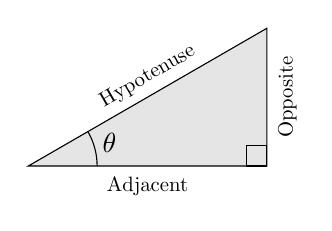
\begin{tikzpicture}[scale=1.75]
					\coordinate (a) at (0, 0);
					\coordinate (b) at ({sqrt(3)}, 0);
					\coordinate (c) at ({sqrt(3)}, 1);
					\draw[fill=gray!20] (a) -- (b) -- (c) -- cycle;
					\node at (0.866, -0.15)[scale=0.75] {Adjacent};
					\node at (1.882, 0.5)[scale=0.75,rotate=90] {Opposite};
					\node at (0.866, 0.65)[scale=0.75,rotate=30] {Hypotenuse};
					\draw (1.582, 0) rectangle (1.732, 0.15);
					\draw (0.5, 0) arc (0:30:0.5);
					\node at (0.46985, 0.171)[scale=1,right]{$\theta$};
				\end{tikzpicture}
			\item[] 
				\begin{flalign*}
					\llap{$\sin{\theta}$} &= \frac{\textrm{opp}}{\textrm{hyp}} \quad
							\csc{\theta} = \frac{\textrm{hyp}}{\textrm{opp}} &\\
					\llap{$\cos{\theta}$} & = \frac{\textrm{adj}}{\textrm{hyp}} \quad
							\sec{\theta}  = \frac{\textrm{hyp}}{\textrm{adj}} &\\
					\llap{$\tan{\theta}$} & = \frac{\textrm{opp}}{\textrm{adj}} \quad
							\cot{\theta}  = \frac{\textrm{adj}}{\textrm{opp}} &
				\end{flalign*}
		\end{enumerate} \end{multicols}
	\item[]
		\begin{multicols}{2} \begin{enumerate}
			\item[]
				%% CIRCLE AND ANGLE DIAGRAM %%
				\hspace{-0.7cm}
				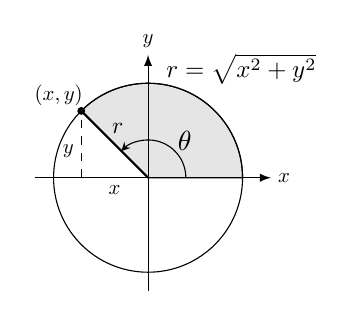
\begin{tikzpicture}[scale=1.2,>=latex]
					% Fill the circle-sector
					\draw[fill=gray!20] (0, 0) -- (1, 0) arc (0:135:1) -- cycle;
					\draw (0, 0) circle(1);
					\draw[->,thin] (-1.2, 0) -- (1.3, 0) node[scale=0.75,right]{$x$};
					\draw[->,thin] (0, -1.2) -- (0, 1.3) node[scale=0.75,above]{$y$};
					\draw[thick] (0, 0) -- (135:1);
					\draw (130:0.5) node[above,scale=0.85]{$r$};
					\filldraw[black] (135:1) circle(1pt);
					\draw (125:1.07) node[left,scale=0.75]{$(x,y)$};
					\draw[dashed] ({cos(135)}, 0) -- ({cos(135)}, {sin(135)});
					\draw ({cos(135)}, {0.40*sin(135)}) node[scale=0.75,left] {$y$};
					\draw ({0.5*cos(135)}, 0) node[scale=0.75,below]{$x$};
					\draw[>=stealth,->] (0.4, 0) arc (0:135:0.4);
					\node at (45:0.55) [scale=1]{$\theta$};
					\node at (0.1, 1.15) [scale=0.9,right]{$r=\sqrt{x^2 + y^2}$};			
				\end{tikzpicture}
			\item[]
				\begin{flalign*}
					\llap{$\sin{\theta}$} &= \frac{y}{r} \quad \csc{\theta} = \frac{r}{y} &\\
					\llap{$\cos{\theta}$} &= \frac{x}{r} \quad \sec{\theta} = \frac{r}{x} &\\
					\llap{$\tan{\theta}$} &= \frac{y}{x} \quad \cot{\theta} = \frac{x}{y} & \\
					\phantom{a} &
				\end{flalign*}
		\end{enumerate} \end{multicols}
	\item[]
		%% UNIT CIRCLE %%
		\phantom{a} 
		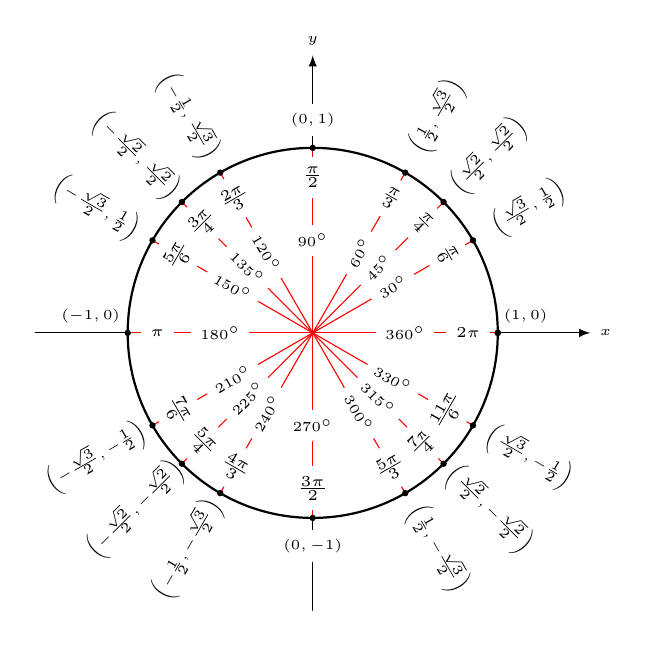
\begin{tikzpicture}[scale=2.35,cap=round,>=latex]
			% Shrink text for this sheet
			\tikzstyle{every node}=[font=\tiny]

			% draw the axes
			\draw[->] (-1.5, 0) -- (1.5, 0) node[right,fill=white] {$x$};
			\draw[->] (0, -1.5) -- (0, 1.5) node[above,fill=white] {$y$};
			% Draw the unit circle
			\draw[thick] (0, 0) circle(1);
			% Draw and label spokes and draw dots on circle's circumference
			% x: angle, xang: rotation of label
			\foreach \x / \xang in
			{
				0 / 0,
				30 / 30,
				45 / 45,
				60 / 60,
				90 / 0,
				120 / -60,
				135 / -45,
				150 / -30,
				180 / 0,
				210 / 30,
				225 / 45,
				240 / 60,
				270 / 0,
				300 / -60,
				315 / -45,
				330 / -30,
				360 / 0
			} {
				% Lines from center to point
				\draw[red] (0, 0) -- (\x:1);
				% Dots at each angle
				\filldraw[black] (\x:1) circle(0.4pt);
				% Draw each angle and label with degrees. Rotate label by xang
				\draw (\x:0.5) node[scale=1.0,fill=white,rotate=\xang] {$\x^\circ$};
			}
			% label each angle in radians
			% x: angle, xtext: radian label, xang: rotation of label
			\foreach \x / \xtext / \xang in
			{
				30 / \frac{\pi}{6} / -60,
				45 / \frac{\pi}{4} / -45,
				60 / \frac{\pi}{3} / -30,
				90 / \frac{\pi}{2} / 0,
				120 / \frac{2\pi}{3} / 30,
				135 / \frac{3\pi}{4} / 45,
				150 / \frac{5\pi}{6} / 60,
				180 / \pi / 0,
				210 / \frac{7\pi}{6} / -60,
				225 / \frac{5\pi}{4} / -45,
				240 / \frac{4\pi}{3} / -30,
				270 / \frac{3\pi}{2} / 0,
				300 / \frac{5\pi}{3} / 30,
				315 / \frac{7\pi}{4} / 45,
				330 / \frac{11\pi}{6} / 60,
				360 / 2\pi / 0
			} {
				\draw (\x:0.84) node[scale=1.1,fill=white,rotate=\xang] {$\xtext$};
			}
			% place Cartesian coordinates around circle
			% x: angle, xtext: x value, ytext: y value, xang: label rotation angle
			\foreach \x / \xtext / \ytext / \xang in
			{
				% the coordinates for the first quadrant
				30 / \frac{\sqrt{3}}{2} / \frac{1}{2} / 30,
				45 / \frac{\sqrt{2}}{2} / \frac{\sqrt{2}}{2} / 45,
				60 / \frac{1}{2} / \frac{\sqrt{3}}{2}/60,
				% The coordinates for the second quadrant
				120 / -\frac{1}{2} / \frac{\sqrt{3}}{2} / -60,
				135 / -\frac{\sqrt{2}}{2} / \frac{\sqrt{2}}{2} / -45,
				150 / -\frac{\sqrt{3}}{2} / \frac{1}{2} / -30, 
				% The coordinates for the third quadrant
				210 / -\frac{\sqrt{3}}{2} / -\frac{1}{2} / 30,
				225 / -\frac{\sqrt{2}}{2} / -\frac{\sqrt{2}}{2} / 45,
				240 / -\frac{1}{2} / -\frac{\sqrt{3}}{2} / 60,
				% The coordinates for the fourth quadrant
				300 / \frac{1}{2} / -\frac{\sqrt{3}}{2} / -60,
				315 / \frac{\sqrt{2}}{2} / -\frac{\sqrt{2}}{2} / -45,
				330 / \frac{\sqrt{3}}{2} / -\frac{1}{2} / -30
			} {
				\draw (\x:1.35) node[rotate=\xang] {$\left( \xtext, \ytext \right)$};
			}
			% Label the circle's intersections with the axes
			\draw (-1.2, 0) node[above=0.2pt] {$(-1,0)$};
			\draw (1.15, 0) node[above=0.2pt] {$(1,0)$};
			\draw (0, -1.15) node[fill=white] {$(0,-1)$};
			\draw (0, 1.15) node[fill=white] {$(0,1)$};
		\end{tikzpicture}
\end{enumerate} \end{multicols}  % P1_DIAGRAMS

%% Page #1 Trig Identities %%
% Two columns for identities
\begin{multicols}{2} \begin{enumerate}  % P1_TRIG_IDENTITIES
	\item[] 
		\textbf{\underline{Reciprocal Identities}}
		\begin{flalign*}
			\sin{\theta} &= \frac{1}{\csc{\theta}} \quad
					\cos{\theta} = \frac{1}{\sec{\theta}} \quad
					\tan{\theta} = \frac{1}{\cot{\theta}} &\\
			\csc{\theta} &= \frac{1}{\sin{\theta}} \quad
					\sec{\theta} = \frac{1}{\cos{\theta}} \quad
					\cot{\theta} = \frac{1}{\tan{\theta}} &
		\end{flalign*}
	\item[] 
		\textbf{\underline{Tangent and Cotangent Identities}}
		\begin{flalign*}
			\tan{\theta} &= \frac{\sin{\theta}}{\cos{\theta}} \quad 
					\cot{\theta} = \frac{\cos{\theta}}{\sin{\theta}} &
		\end{flalign*}
	\item[] 
		\textbf{\underline{Pythagorean Identities}}
		\begin{flalign*}
			\sin^2{\theta} + \cos^2{\theta} = 1 \quad & \phantom{a} &\\
			1 + \tan^2{\theta} = \sec^2{\theta} \quad & 1 + \cot^2{\theta} = \csc^2{\theta} &
		\end{flalign*}
	\item[] 
		\textbf{\underline{Cofunction Identities}}
		\begin{flalign*}
			&\sin{\left(\frac{\pi}{2} - \theta \right)} = \cos{\theta}  \quad
					\cos{\left(\frac{\pi}{2} - \theta \right)} = \sin{\theta} & \\
			&\csc{\left(\frac{\pi}{2} - \theta \right)} = \sec{\theta}  \quad
					\tan{\left(\frac{\pi}{2} - \theta \right)} = \cot{\theta} & \\
			&\sec{\left(\frac{\pi}{2} - \theta \right)} = \csc{\theta}  \quad
					\cot{\left(\frac{\pi}{2} - \theta \right)} = \tan{\theta} & 
		\end{flalign*}
	\item[] 
		\textbf{\underline{Reduction Formulas}}
		\begin{flalign*}
			&\sin{(-\theta)} = -\sin{\theta} \quad \,\cos{(-\theta)} = \cos{\theta} & \\
			&\csc{(-\theta)} = -\csc{\theta} \quad \tan{(-\theta)} = -\tan{\theta} & \\
			&\sec{(-\theta)} = \sec{\theta} \qquad  \cot{(-\theta)} = -\cot{\theta} &
		\end{flalign*}
	\item[] 
		\textbf{\underline{Sum and Difference Formulas}}
		\begin{flalign*}
			\sin{(\theta \pm \phi)} &= \sin{\theta} \cos{\phi} \pm \cos{\theta} \sin{\phi} & \\
			\cos{(\theta \pm \phi)} &= \cos{\theta} \cos{\phi} \mp \sin{\theta} \sin{\phi} & \\
			\tan{(\theta \pm \phi)} &= \frac{\tan{\theta} \pm \tan{\phi}}{1 \mp \tan{\theta} \tan{\phi}} &
		\end{flalign*}
	\item[] 
		\textbf{\underline{Double-Angle Formulas}}
		\begin{flalign*}
			\sin{2\theta} &= 2 \sin{\theta}\cos{\theta} & \\
			\cos{2\theta} &= \cos^2{\theta} - \sin^2{\theta} = 2\cos^2{\theta} - 1 = 1 - 2\sin^2{\theta} & \\
			\tan{2\theta} &= \frac{2\tan{\theta}}{1 - \tan^2{\theta}} &
		\end{flalign*}
	\item[] 
		\textbf{\underline{Power-Reducing Formulas}}
		\begin{flalign*}
			\sin^2{\theta} &= \frac{1}{2}(1 - \cos{2 \theta}) & \\
			\cos^2{\theta} &= \frac{1}{2} (1 + \cos{2\theta}) & \\
			\tan^2{\theta} &= \frac{1- \cos{2\theta}}{1 + \cos{2 \theta}} & 
		\end{flalign*}
	\item[] 
		\textbf{\underline{Sum-to-Product Formula}}
		\begin{flalign*}
			\sin{\theta} + \sin{\phi} &= 2 \sin{\left( \frac{\theta + \phi}{2} \right)}
					\cos{\left( \frac{\theta - \phi}{2} \right)} & \\
			\sin{\theta} - \sin{\phi} &= 2 \cos{\left( \frac{\theta + \phi}{2} \right)}
					\sin{\left( \frac{\theta - \phi}{2} \right)} & \\
			\cos{\theta} + \cos{\phi} &= 2 \cos{\left( \frac{\theta + \phi}{2} \right)}
					\cos{\left( \frac{\theta - \phi}{2} \right)} & \\
			\cos{\theta} - \cos{\phi} &= - 2 \sin{\left( \frac{\theta + \phi}{2} \right)}
					\sin{\left( \frac{\theta - \phi}{2} \right)} & 
		\end{flalign*}
	\item[] 
		\textbf{\underline{Product-to-Sum Formulas}}
		\begin{flalign*}
			\sin{\theta}\sin{\phi} &= \frac{1}{2} \left[ \cos{(\theta - \phi)} - 
					\cos{(\theta + \phi)} \right] & \\
			\cos{\theta}\cos{\phi} &= \frac{1}{2} \left[ \cos{(\theta - \phi)} +
					\cos{(\theta + \phi)} \right] & \\
			\sin{\theta}\cos{\phi} &= \frac{1}{2} \left[ \sin{(\theta + \phi)} +
					\sin{(\theta - \phi)} \right] & \\
			\cos{\theta}\sin{\phi} &= \frac{1}{2} \left[ \sin{(\theta + \phi)} -
					\sin{(\theta - \phi)} \right] &
		\end{flalign*}
\end{enumerate} \end{multicols}  % P1_TRIG_IDENTITIES
% Small vertical buffer
\phantom{a} \vspace{-0.6cm}
\end{minipage}} \end{center}

\newpage

%%% PAGE #2 %%%
\section*{\centering{\underline{DERIVATIVES AND INTEGRALS}}}

\begin{center}
% Box around page 2 content
\fbox{
% Use minipage for page 2 content
\begin{minipage}{0.98\textwidth}
	%% DERIVATIVES %%
	\phantom{a} %\vspace{-0.1cm}
	\textbf{\underline{Basic Differentiation Rules}}
	\begin{multicols}{3} \begin{enumerate}
		\item \ddx{cu} = $cu'$
		\item \ddx{u \pm v} = \m{u' \pm v'}
		\item \ddx{uv} = \m{uv' + u'v}
	 	\item \ddx{\dfrac{u}{v}} = \m{\dfrac{u'v - uv'}{v^2}}
		\item \ddx{c} = \m{0}
		\item \ddx{u^n} = \m{nu^{n-1}u'}
		\item \ddx{x} = 1
		\item \ddx{| u |} = \m{\dfrac{u}{| u |} (u'), \quad u \ne 0}
		\item \ddx{\ln{u}} = \m{\dfrac{u'}{u}}
		\item \ddx{e^u} = \m{e^u u'}
		\item \ddx{\log_a{u}} = \m{\dfrac{u'}{(\ln{a}) u}}
		\item \ddx{a^u} = \m{(\ln{a}) a^u u'}	
		\item \ddx{\sin{u}} = \m{(\cos{u})u'}
		\item \ddx{\cos{u}} = \m{-(\sin u)u'}
		\item \ddx{\tan u} = \m{(\sec^2 u)u'}
		\item \ddx{\cot u} = \m{-(\csc^2 u) u'}
		\item \ddx{\sec u} = \m{(\sec u\, \tan u)u'}
		\item \ddx{\csc u} = \m{-(\csc u\, \cot u)u'}
		\item \ddx{\arcsin u} = \m{\dfrac{u'}{\sqrt{1 - u^2}}}
		\item \ddx{\arccos u } = \m{\dfrac{-u'}{\sqrt{1 - u^2}}}
		\item \ddx{\arctan u} = \m{\dfrac{u'}{1 + u^2}}
		\item \ddx{\arccot u} = \m{\dfrac{-u'}{1 + u^2}}
		\item \ddx{\arcsec u } = \m{\dfrac{u'}{| u |\sqrt{u^2 - 1}}}
		\item \ddx{\arccsc u} = \m{\dfrac{-u'}{| u |\sqrt{u^2 - 1}}}
		\item \ddx{\sinh u} = \m{(\cosh u)u'}
		\item \ddx{\cosh u} =\m{(\sinh u) u'}
		\item \ddx{\tanh u } = \m{(\sech^2 u) u'}
		\item \ddx{\coth} = \m{-(\csch^2 u)u'}
		\item \ddx{\sech u} = \m{-(\sech u \, \tanh u)u'}
		\item \ddx{\csch u} = \m{-(\csch u\, \coth u)u'}
		\item \ddx{\sinh^{-1} u} = \m{\dfrac{u'}{\sqrt{u^2 + 1}}}
		\item \ddx{\cosh^{-1} u} = \m{\dfrac{u'}{\sqrt{u^2 - 1}}}
		\item \ddx{\tanh^{-1} u} = \m{\dfrac{u'}{1 - u^2}}
		\item \ddx{\coth^{-1} u} = \m{\dfrac{u'}{1 - u^2}}
		\item \ddx{\sech^{-1} u} = \m{\dfrac{-u'}{u \sqrt{1 - u^2}}}
		\item \ddx{\csch^{-1} u} = \m{\dfrac{-u'}{| u | \sqrt{1 + u^2}}}
	\end{enumerate}\end{multicols}

	%% INTEGRALS %%
	\phantom{a}
	\textbf{\underline{Basic Integration Formulas}}
	\begin{multicols}{2} \begin{enumerate}
		\item \m{\int \! kf(u) \, du} = \m{k \int \! f(u) \, du}
		\item \m{\int \! [f(u) \: \pm \: g(u)] \,du} = \m{\int \! f(u)\,du \: \pm \: \int\! g(u) \,du}
		\item \m{ \int  du} = \m{u + C}
		\item \m{\int \! a^u \,du} = \m{\left(\dfrac{1}{\ln a} \right) a^u + C}
		\item \m{\int \! e^u \, du} = \m{e^u + C}
		\item \m{\int \! \sin u \,du} = \m{-\cos u + C}
		\item \m{\int \! \cos u \,du} = \m{\sin u + C}
		\item \m{\int \! \tan u \,du} = \m{-\ln{|\cos u|} +C}
		\item \m{\int \! \cot u \, du} = \m{\ln{|\sin u| + C}}
		\item \m{\int \! \sec u \,du} = \m{\ln{|\sec u + \tan u|} + C}
		\item \m{\int \! \csc u \, du} = \m{-\ln{|\csc u + \cot u| + C}}
		\item \m{\int \! \sec^2 \, du} = \m{\tan u + C}
		\item \m{\int \! \csc^2 u \, du} = \m{-\cot u + C }
		\item \m{\int \! \sec u \tan u \, du} = \m{\sec u + C}
		\item \m{\int \! \csc u \cot u \, du} = \m{-\csc u + C}
		\item \m{\int \! \dfrac{du}{\sqrt{a^2 - u^2}}} = \m{\arcsin\left( \dfrac{u}{a} \right) + C}
		\item \m{\int \! \dfrac{du}{a^2 + u^2}} = \m{\dfrac{1}{a}\arctan\left( \frac{u}{a} \right) + C}
		\item \m{\int \! \dfrac{du}{u \sqrt{u^2 - a^2}}} = \m{\dfrac{1}{a}\arcsec\left( \dfrac{|u|}{a} \right) + C}	
	\end{enumerate}\end{multicols}	
	\phantom{a} \vspace{-0.2cm}
\end{minipage} } \end{center}

\end{document}
